%%%% fatec-article.tex, 2024/03/10

%% Classe de documento
\documentclass[
  a4paper,%% Tamanho de papel: a4paper, letterpaper (^), etc.
  12pt,%% Tamanho de fonte: 10pt (^), 11pt, 12pt, etc.
  english,%% Idioma secundário (penúltimo) (>)
  brazilian,%% Idioma primário (último) (>)
]{article}

%% Pacotes utilizados
\usepackage[]{fatec-article}
\usepackage{graphicx}
\usepackage{float}

\Author{1}{Name={Amanda de Oliveira Costa\\ Arthur Ribeiro Dias Fudali \\ Diego Baltazar de Souza Claudio \\ Giovana da Silva Albanês Santos \\ Igor Leite Gomes }}

\Author{2}{Name={\{ amanda.costa47@fatec.sp.gov.br  \}\\ \{ arthur.fudali@fatec.sp.gov.br \} \\ \{ diego.claudio@fatec.sp.gov.br\} \\ \{ giovana.santos30@fatec.sp.gov.br \} \\ \{ igor.gomes4@fatec.sp.gov.br \}}}

%% Definição das palavras-chaves/keywords
\Keyword{1}{TDA}{ADHD}
\Keyword{2}{atenção}{attention}
\Keyword{3}{rastreamento ocular}{eye tracking}
\Keyword{4}{gamificação}{gamification}
\Keyword{5}{ODS 3}{SDG 3}

%%%% Resumo no idioma primário (brazilian)
\begin{Abstract}[brazilian]%% Idioma (brazilian ou english)
O Transtorno de Déficit de Atenção (TDA) é uma condição neuropsicológica que pode
afetar significativamente o desempenho de adultos em diversas esferas da vida, como
trabalho, estudos e relações interpessoais. O diagnóstico tradicional envolve avaliações
clínicas e testes padronizados, os quais nem sempre estão disponíveis de forma acessível ou
apresentam dados objetivos suficientes para um rastreio inicial eficaz. Este estudo propõe
uma abordagem tecnológica que integra uma plataforma digital gamificada, baseada no
Teste de Desempenho Contínuo (TDC), com técnicas de rastreamento ocular em tempo real.
A proposta tem como objetivo identificar possíveis indícios de TDA em adultos por meio da
análise de desempenho atencional durante a execução de tarefas gamificadas. O sistema
registra dados como tempo de reação, erros de omissão e comissão, variabilidade nas
respostas e padrões de fixação ocular, os quais são processados automaticamente. Com base
na comparação com bases de dados normativas, o sistema fornece um feedback
interpretativo ao usuário, podendo contribuir como ferramenta complementar de triagem
inicial. A acessibilidade da plataforma, que roda diretamente no navegador, e seu caráter
lúdico e autônomo tornam a solução promissora para ampliar o acesso ao rastreamento
precoce de indícios do transtorno. A proposta está alinhada ao terceiro Objetivo de
Desenvolvimento Sustentável (ODS) da Agenda 2030 da ONU, que visa garantir saúde e
bem-estar para todas as pessoas, promovendo inovações tecnológicas para uma saúde mais
inclusiva, eficiente e orientada por dados objetivos.
\end{Abstract}

%%%% Resumo no idioma secundário (english)
\begin{Abstract}[english]%% Idioma (brazilian ou english)
Attention Deficit Disorder (ADD) is a neuropsychological condition that can
significantly affect adults' performance in various areas of life, such as work, studies, and
interpersonal relationships. Traditional diagnosis involves clinical evaluations and standardized
tests, which are not always accessible or provide sufficient objective data for effective initial
screening. This study proposes a technological approach that integrates a gamified digital
platform, based on the Continuous Performance Test (CPT), with real-time eye tracking
techniques. The proposal aims to identify possible signs of ADD in adults by analyzing
attentional performance during the execution of gamified tasks. The system records data
such as reaction time, omission and commission errors, response variability, and eye fixation
patterns, which are processed automatically. Based on comparison with normative databases,
the system provides interpretative feedback to the user, and can contribute as a
complementary tool for initial screening. The accessibility of the platform, which runs directly
in the browser, and its playful and autonomous nature make it a promising solution for
expanding access to early screening for signs of the disorder. The proposal is aligned with the
third Sustainable Development Goal (SDG) of the UN 2030 Agenda, which aims to ensure
health and well-being for all people, promoting technological innovations for more inclusive,
efficient health care guided by objective data.
\end{Abstract}

%% Processamento de entradas (itens) do índice remissivo (makeindex)
\makeindex%

%% Arquivo(s) de referências
\addbibresource{fatec-article.bib}

%% Início do documento
\begin{document}

% Seções e subseções
%\section{Título de Seção Primária}%

%\subsection{Título de Seção Secundária}%

%\subsubsection{Título de Seção Terciária}%

%\paragraph{Título de seção quaternária}%

%\subparagraph{Título de seção quinária}%

\section*{Introdução}%
\label{sect:intro}
A Organização das Nações Unidas (ONU) estabelece, por meio da Agenda 2030, metas para promover o desenvolvimento sustentável e o bem-estar global. Entre os 17 Objetivos de Desenvolvimento Sustentável (ODS), o terceiro busca garantir saúde de qualidade e promover o bem-estar para todos. Nesse contexto, este trabalho visa contribuir para essa meta ao propor uma solução tecnológica voltada à identificação de indícios do Transtorno de Déficit de Atenção (TDA) em adultos.\textcite{unitednations2015agenda2030}

O TDA é uma condição neurobiológica de causas genéticas, que afeta milhões de pessoas em todo o mundo. É caracterizada por sintomas de
desatenção, impulsividade, e, em alguns casos, hiperatividade, afetando significativamente o
desempenho acadêmico, profissional e social dos afetados. Embora o diagnóstico clínico do
TDA seja baseado tradicionalmente em entrevistas e questionários subjetivos, avanços
tecnológicos têm permitido o uso de ferramentas mais robustas e quantitativas para apoiar
esse processo. \textcite{BVS2014}
Entre essas ferramentas, destaca-se o \textit{eye tracking} (do português, rastramento ocular), esta é uma técnica
que consiste em usar o posicionamento dos olhos de uma pessoa para obter informações
sobre onde ela está olhando. Isso pode ser feito usando luzes infravermelhas, que calculam
exatamente onde a pessoa está olhando com base nas reflexões da luz na retina, ou por
meio de câmeras que monitoram visualmente a posição dos olhos e identificam sua direção.

Em ambientes controlados, o teste com \textit{eye tracking} envolve a realização de tarefas
padronizadas, nas quais o comportamento visual do participante é monitorado sem
interferência direta de um moderador. Essa abordagem objetiva permite uma coleta mais
confiável de dados, reduzindo o viés associado ao autorrelato e aumentando a credibilidade
da análise. Além disso, a comparação dos dados obtidos com padrões normativos permite
identificar desvios significativos no desempenho visual atencional, muitas vezes
imperceptíveis a métodos tradicionais.

Quando aplicada em um teste diagnóstico, a técnica permite acompanhar com
precisão os movimentos dos olhos de um indivíduo durante a realização de tarefas
específicas, fornecendo dados objetivos e detalhados sobre onde, por quanto tempo e em
que sequência uma pessoa fixa seu olhar em determinados estímulos visuais. Estudos
demonstram que pessoas com TDA apresentam menor tempo de fixação e padrão visual
mais disperso ao realizarem testes de desempenho, sugerindo dificuldade em manter a
atenção sustentada e filtragem de estímulos irrelevantes \textcite{Lim2024}.

A Inteligência Artificial (IA) surge como um campo essencial nesse contexto, voltado à criação de sistemas capazes de simular aspectos da cognição humana, como percepção, raciocínio, aprendizado e tomada de decisão. Segundo \textcite{sep-chinese-room}, a IA pode ser dividida em dois tipos: IA Forte, capaz de compreender e raciocinar de forma semelhante aos humanos; e IA Fraca, restrita à execução de tarefas específicas sem capacidade de raciocínio autônomo. O avanço dessas tecnologias, apoiado por algoritmos de aprendizagem profunda, processamento de linguagem natural e análise de dados, tem permitido desenvolver sistemas cada vez mais precisos e adaptativos.

Associada à IA, a Internet das Coisas (Internet of Things, IoT) amplia o potencial de integração tecnológica ao conectar dispositivos físicos, como sensores e equipamentos inteligentes, à internet. Essa interconexão possibilita a coleta, o compartilhamento e a análise de dados em tempo real, criando ecossistemas inteligentes baseados em computação em nuvem e comunicação entre máquinas. \textcite{IEEE}
 
O Teste de Desempenho Contínuo (TDC) é uma medida padronizada amplamente
utilizada na neuropsicologia para avaliar métricas de atenção sustentada, impulsividade,
tempo de resposta e variabilidade dos tempos de reação. Trata-se de uma tarefa
computadorizada na qual o usuário responde e reage a estímulos apresentados
sequencialmente, permitindo medidas de desempenho atencional ao longo do tempo. 
A atenção é um processo cognitivo complexo que envolve diferentes componentes inter-relacionados, essenciais para o desempenho em tarefas como o teste de desempenho contínuo. De forma geral, pode ser classificada em quatro tipos principais. A atenção sustentada refere-se à capacidade de manter o foco em um estímulo ou tarefa por um período prolongado, sendo fundamental para evitar erros de omissão no TDC. A atenção seletiva envolve a habilidade de concentrar-se em informações relevantes enquanto se ignora distrações, o que influencia diretamente a precisão das respostas. A atenção alternada diz respeito à flexibilidade cognitiva para mudar o foco entre diferentes estímulos ou tarefas, demonstrando controle executivo. Por fim, a atenção dividida representa a capacidade de processar simultaneamente múltiplas fontes de informação, exigindo coordenação eficiente de recursos cognitivos. A compreensão dessas modalidades permite interpretar de forma mais abrangente as métricas obtidas no TDC.\textcite{CULLUM1998303}

Os \textit{serious games} (jogos sérios) também vêm se destacando como ferramentas complementares em contextos de avaliação e reabilitação cognitiva. Esses jogos digitais, desenvolvidos com finalidades que vão além do entretenimento, oferecem ambientes interativos e imersivos que aumentam o engajamento do usuário e permitem mensurar habilidades cognitivas de forma dinâmica.

Desta forma,a integração entre eye tracking, IA e jogos sérios representa uma abordagem promissora para a triagem e o apoio diagnóstico do TDA.
A análise dos dados com IA pode indicar o grau de
desatenção apresentado por um indivíduo em diferentes contextos e contribuir para decisões
clínicas mais embasadas. Assim, este estudo propõe o desenvolvimento de um software gamificado que utilize informações de rastreamento ocular processadas com base nas métricas do TDC, a fim de gerar um indicador do desempenho atencional geral e oferecer uma possível estimativa preliminar para o Transtorno de Déficit de Atenção.

\section*{OBJETIVO} \label{sect:obj}

Desenvolver uma plataforma digital gamificada, acessível por navegador, que utiliza
rastreamento ocular e métricas de desempenho atencional para auxiliar na triagem inicial de
indícios do TDA em crianças de 10 a 12 anos.

\subsection*{OBJETIVOS ESPECÍFICOS} 

\begin{itemize}
    \item Integrar o TDC a um jogo digital com tarefas que
    simulam desafios atencionais.
    \item  Aplicar técnicas de \textit{eye tracking} em tempo real para registrar padrões de
    atenção durante a execução das tarefas.
    \item Processar automaticamente os dados coletados e compará-los com parâmetros
    normativos para gerar feedback ao usuário.
    \item Promover uma solução acessível, autônoma e alinhada ao ODS 3 da ONU, que amplie
    o acesso à triagem inicial de TDA.
\end{itemize}


\section*{ESTADO DA ARTE} \label{sect:estadoarte}

Nesta seção, você deverá realizar um mapeamento de toda a produção acadêmica sobre o tema do seu projeto. É um processo bastante importante porque reúnem todas as pesquisas e descrevem as conclusões das pesquisas sobre o tema \cite{smith:99}. Para escrever um bom estado da arte, você poderá utilizar algumas perguntas norteadoras, tais como:

\begin{enumerate}
    \item O que as atuais pesquisas científicas concluíram sobre o tema?
    \item Quais as divergências dos pesquisadores sobre o assunto?
    \item Quem está pesquisando sobre esse tema?
    \item Onde estão fazendo essas pesquisas?
\end{enumerate}

Em outras palavras, o estado da arte destaca os aspectos de outras pesquisas, mas também identifica as lacunas que existem nessas pesquisas. Ou seja: analisa o que as pesquisas falaram e o que não falaram sobre o tema \cite{Alencar2007,Beltrano2021,Fulano2021}.

Segundo \textcite{Ramos2003,Carvalho2004}, para que você possa descrever as pesquisas/trabalhos que estão relacionados ao seu, não esqueça de citá-los ao decorrer do texto. Para isso, você poderá utilizar o comando $\backslash$cite para citação implícita ou o comando $\backslash$textcite para citações explícitas.

As citações diretas curtas (de até três linhas) acompanham o corpo do texto e se destacam com aspas duplas. Caso o texto original já contenha aspas, estas devem ser substituídas por aspas simples. Enquanto que, para representar as citações diretas longas (com mais de três linhas), estas devem ser transcritas em parágrafo distinto, da seguinte forma:

\begin{displayquote}
   Toda citação direta com mais de três linhas é considerada uma citação direta longa.
Este tipo de citação deve ser escrita sem aspas, em parágrafo distinto, com fonte de tamanho 10, espaçamento simples e com recuo de 4cm da margem esquerda, terminando na margem direita, conforme ilustrado neste exemplo \cite{Andujar2006}.
\end{displayquote}

Vale ressaltar que a utilização de citações diretas longas deve ser evitada durante a escrita de artigos científicos. Conforme visto em \textcite{Kalakota2002,Purcidonio2008}, os dados de cada referência podem ser obtidos de um arquivo com a extensão bib, geralmente na própria página de \textit{download} da referência (artigos, livros, etc.) ou, ainda, a partir do Google Acadêmico, etc.



\section*{METODOLOGIA} \label{sect:metodologia}

A seção de Metodologia explica aos leitores quais procedimentos, abordagens, desenhos e tratamento realizamos na pesquisa, o que permitirá replicar os estudos, entender a linearidade entre a abordagem dos objetivos e os resultados obtidos, determinar sua adequação e relevância e evidenciar qualquer viés na maneira como o estudo foi elaborado e realizado. Em outras palavras, é uma estrutura contextual que apresenta um caminho lógico para responder a perguntas que você levanta no início de sua tese ou artigo \cite{knuth:84}. 

É importante que nesta seção, você descreva todas as ferramentas e tecnologias utilizadas para o desenvolvimento da sua pesquisa \cite{boulic:91}. Lembre-se de detalhar para que serve cada ferramenta e tecnologia e o motivo da sua escolha.


% \section*{RESULTADOS PRELIMINARES}\label{sect:resultados}%

%O propósito da seção de resultados, como o próprio nome indica, é revelar o que foi encontrado na pesquisa. Essa parte do artigo estará composta dos dados relevantes obtidos e sintetizados pelo autor. 

Nesta seção, você deverá apresentar todos os elementos solicitados no mapa mental relacionados ao seu projeto: diagramas, protótipos, modelo de negócios, principais funções e componentes desenvolvidos. Para tanto, na subseção a seguir, você poderá consultar como é feita a inserção de figuras, fluxogramas, fotografias, gráficos, tabelas e quadros.

\subsection*{Ilustração e Tabela}

Independentemente da ilustração (figura, fluxograma, fotografia, gráfico, quadro, entre outras) ou tabela inserida no trabalho, sua identificação deve aparecer na parte superior. Esta identificação deve ser precedida da palavra designativa, seguida de seu número de ordem de ocorrência no texto, em algarismos arábicos, travessão e do respectivo título.

Após a ilustração ou tabela, na parte inferior, indicar a fonte consultada (mesmo sendo produção do próprio autor), legenda, notas e outras informações necessárias à sua compreensão (se houver). A ilustração deve ser citada no texto e inserida o mais próximo possível do trecho a que se refere. A seguir, encontra-se um exemplo para a inserção de um elemento do tipo Gráfico, o \Cref{grph:example}.

\begin{graph}[!h]
\centering
\SetCaptionWidth{\ifbool{@LayoutA}{0.7}{0.72}\linewidth}
\caption{Exemplo de gráfico}%
\label{grph:example}
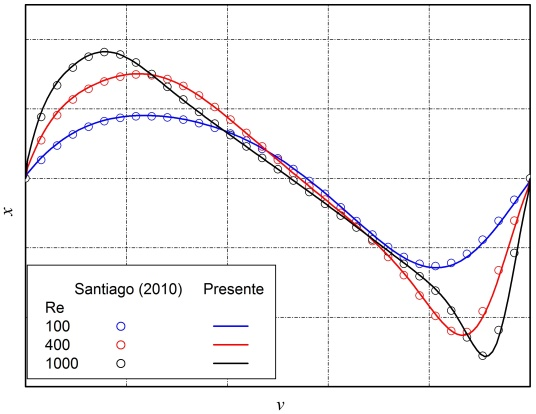
\includegraphics[width = \CaptionWidth]{grph-example}
\SourceOrNote{Autoria Própria (2024)}
\end{graph}

Em computação, é muito comum a utilização de fluxogramas, para documentar, estudar, planejar, melhorar e comunicar processos complexos por meio de diagramas claros e fáceis de entender. Um fluxograma é um diagrama que descreve um processo, sistema ou algoritmo de computador. O \Cref{fcht:ex-algorithm} é um dos vários exemplos deste tipo de ilustração que pode ser gerado ou editado na ferramenta \textit{online} \href{http://www.lucidchart.com/}{Lucidchart}, entre outras.

\begin{flowchart}[!htb]
\centering
\caption{Exemplo de fluxograma de algoritmo}%
\label{fcht:ex-algorithm}
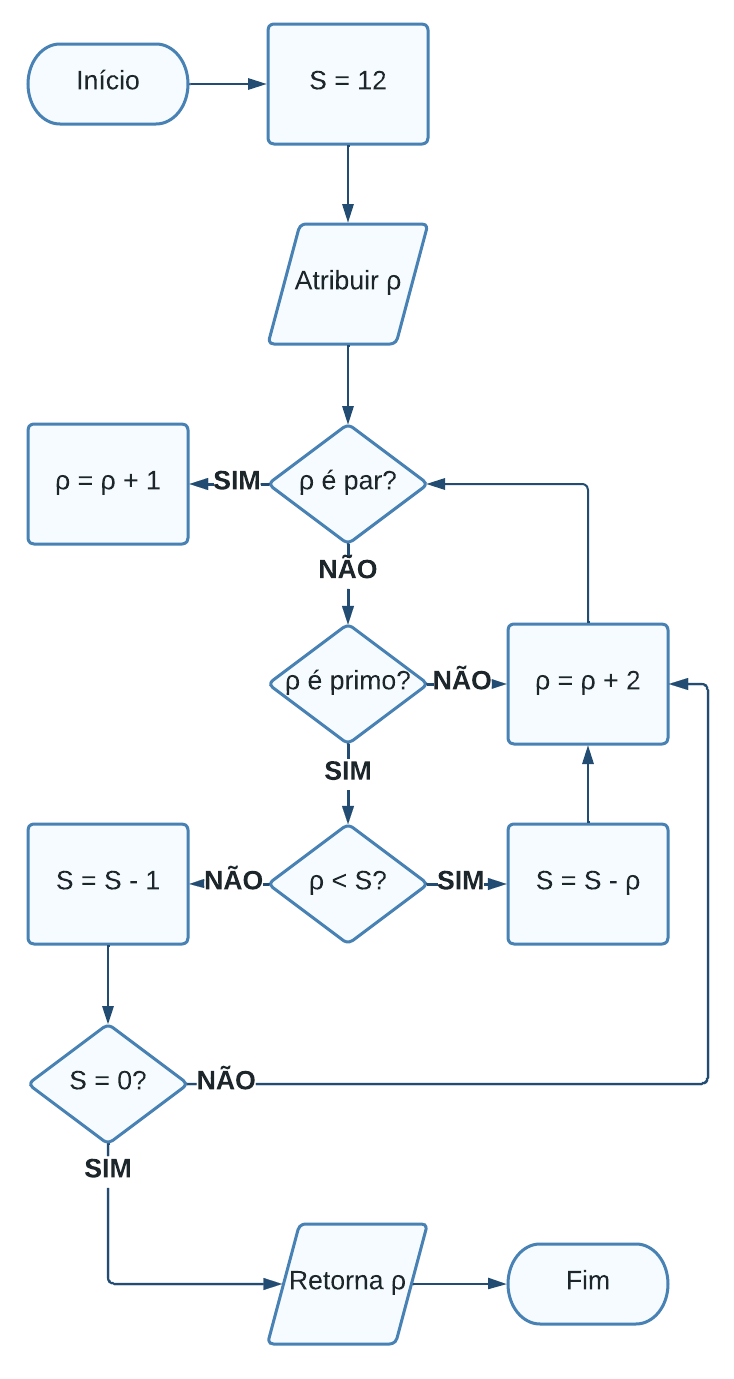
\includegraphics[scale=0.4]{fcht-ex-algorithm}
\SourceOrNote{Autoria Própria (2024)}
\end{flowchart}

O LaTeX tem uma biblioteca específica para utilizar imagens no documento. O pacote graphicx habilita um ambiente chamado figure, que permite que você insira imagens de uma forma simples no texto. A \Cref{fig:example-image-duck} é um exemplo deste tipo de ilustração.

\begin{figure}[!h]
\centering
\caption{Exemplo de figura}%
\label{fig:example-image-duck}
\includegraphics[scale=1.2]{example-image-duck}
\SourceOrNote{Autoria Própria (2024)}
\end{figure}

Caso seja necessário, você ainda poderá inserir fotografias, por meio do ambiente \textit{photograph}, conforme ilustrado na \Cref{phot:pg-campus}.

\begin{photograph}[!h]
\centering
\SetCaptionWidth{\ifbool{@LayoutA}{0.7}{0.72}\linewidth}
\caption{Fachada da Fatec de Registro}%
\label{phot:pg-campus}
\savebox0{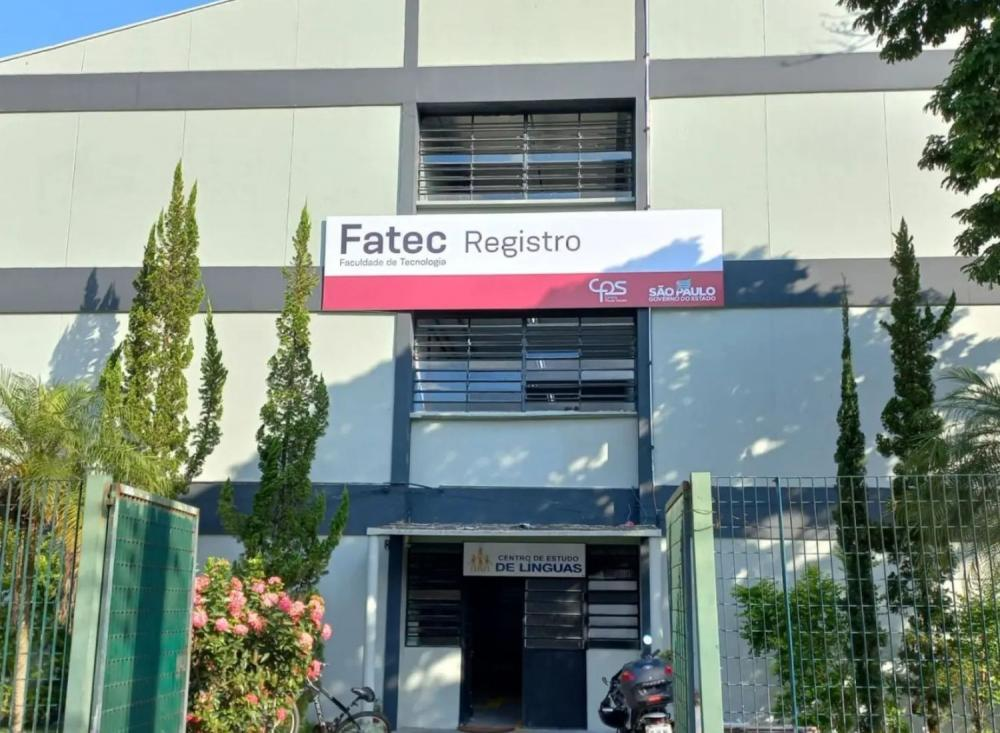
\includegraphics[width = \CaptionWidth]{Illustrations/fachada-fatec.jpg}}
\usebox0%
\SourceOrNote{Autoria Própria (2024)}
\end{photograph}

Outro elemento visual bastante utilizado na seção de Resultados são as tabelas, pois elas fornecem uma estrutura visualmente organizada para apresentar dados, tornando a leitura e a compreensão do conteúdo mais fácil para o leitor. As células, linhas e colunas ajudam a alinhar informações de maneira sistemática.

Para conjuntos de dados comparativos, as tabelas são particularmente úteis. Elas possibilitam a disposição lado a lado de informações relacionadas, facilitando a comparação direta entre diferentes elementos.

Tabelas e quadros devem estar centralizados e conter apenas dados imprescindíveis, evitando-se que sejam muito extensos, não repetindo dados já inseridos no texto, ou vice-versa. O formato de tabela pode ser observado na \Cref{tab:example}.

\begin{table}[!htb]
\centering
\SetCaptionWidth{0.5\linewidth}
\caption{Exemplo de tabela}%
\label{tab:example}
\begin{tabularx}{\CaptionWidth}{@{}XY@{}}
\toprule%
\rowcolor{TableColor}
\multicolumn{1}{Y}{\textcolor{white}{Idade}}           &
\multicolumn{1}{Y}{\textcolor{white}{Percentual (\%)}} \\
\midrule%
Até 20 anos     & 0  \\
De 21 a 30 anos & 10 \\
De 31 a 40 anos & 20 \\
De 41 a 50 anos & 30 \\
\bottomrule%
\end{tabularx}
\SourceOrNote{Adaptada de \textcite{Beltrano2021}}
\end{table}

No caso de quadros, deve ser seguida a estrutura demonstrada no \Cref{tfrm:typography}.
Caso os dados sejam inéditos e provenientes de uma pesquisa realizada pelos próprios autores do trabalho, essa especificação deve constar na fonte com o ano da pesquisa de campo.
Nesse caso, a fonte deve ser: Autoria Própria (2024).

\begin{tabframed}[!htb]
\centering
\caption{Tipografia das seções}%
\label{tfrm:typography}
\begin{tabularx}{\linewidth}{?{}p{20mm}|X|p{45mm}?{}}%% CHKTEX 44
\toprule%
\rowcolor{TableColor}
\multicolumn{1}{?{}c|}{\textcolor{white}{Seção}}   &
\multicolumn{1}{c|}{\textcolor{white}{Tipografia}} &
\multicolumn{1}{c?{}}{\textcolor{white}{Exemplo}}  \\
\midrule%
Primária                     &
Letras maiúsculas em negrito &
\textbf{1 SEÇÃO PRIMÁRIA}    \\
\midrule%
Secundária                    &
Letras maiúsculas sem negrito &
1.1 SEÇÃO SECUNDÁRIA          \\
\midrule%
Terciária                                                             &
Letra inicial de todas as palavras em maiúscula, sem negrito &
1.1.1 Seção Terciária                                                 \\
\midrule%
Quaternária                                                          &
Letra inicial da primeira palavra em maiúscula, sem negrito &
1.1.1.1 Seção quaternária                                            \\
\midrule%
Quinária                                                                          &
Letra inicial da primeira palavra em maiúscula, sem negrito e em itálico &
\textit{1.1.1.1.1 Seção quinária}                                                 \\
\bottomrule%
\end{tabularx}
\SourceOrNote{Autoria Própria (2024)}
\end{tabframed}

Quadros e tabelas podem ser inseridos neste documento usando os ambientes \texttt{tabframed} e \texttt{table}, respectivamente, conforme exemplos no arquivo-fonte deste modelo. A geração ou edição desses elementos visuais pode ser realizada por meio de ferramentas \textit{online}, tais como: \href{http://www.tablesgenerator.com/}{Tables Generator} e \href{http://www.latex-tables.com/}{Latex Tables Editor}, entre outras.

\subsection*{Equações}

Equações podem ser inseridas neste documento usando o ambiente  \texttt{equation}, como ilustrado na \Cref{eq:u}.

\begin{equation}%
\label{eq:u}
u = \beta \operatorname{sen} \left(\pi x\right) \frac{\left(e^{2x} - 1\right) \left(e^y - 1\right)}{\left(e^2 - 1\right) \left(e - 1\right)}
\end{equation}

Símbolos matemáticos (ou equações mais simples) podem ser inseridos ao longo do texto de um parágrafo usando o ambiente do Latex \texttt{math}. É possível ainda, a utilização de ferramentas onlines para a geração ou edição de equações, tais como: \href{http://formulasheet.com/}{Formula Sheet} e \href{http://www.tutorialspoint.com/latex_equation_editor.htm}{Latex Equation Editor}.

%

%\section*{CONCLUSÃO}\label{sect:conclusao}%

%Apresente aqui as conclusões do seu trabalho, verifique se o objetivo foi cumprido, apresenta respostas para o problema da pesquisa, relate as limitações e as recomendações do estudo. Por fim, coloque sugestões para trabalhos futuros. %

\printbibliography

%% Elementos pós-textuais (opcionais): Apêndice e Anexo
%Caso for utilizar, basta retirar o símbolo de % na frente do comando
%%%%% Elementos pós-textuais
%%
%% Glossário, apêndices, anexos e índice remissivo (opcionais).

%% Apêndices
\begin{Appendix}

\section{Título de Apêndice}%
\label{sect:apx-a1}

Exemplo de apêndice (\Cref{sect:apx-a1}) em uma seção de \nameref{sect:appendix}.

\subsection{Título de Seção Secundária de Apêndice}%
\label{ssect:apx-a2}

Exemplo de seção secundária de apêndice (\Cref{ssect:apx-a2}).

\subsubsection{Título de Seção Terciária de Apêndice}%
\label{sssect:apx-a3}

Exemplo de seção terciária de apêndice (\Cref{sssect:apx-a3}).

\paragraph{Título de seção quaternária de Apêndice}%
\label{prgh:apx-a4}

Exemplo de seção quaternária de apêndice (\Cref{prgh:apx-a4}).

\subparagraph{Título de seção quinária de Apêndice}%
\label{sprgh:apx-a5}

Exemplo de seção quinária de apêndice (\Cref{sprgh:apx-a5}).

\end{Appendix}

%% Anexos
\begin{Annex}

\section{Título de Anexo}%
\label{sect:anx-a1}

Exemplo de anexo (\Cref{sect:anx-a1}) em uma seção de \nameref{sect:annex}.

\subsection{Título de Seção Secundária de Anexo}%
\label{ssect:anx-a2}

Exemplo de seção secundária de anexo (\Cref{ssect:anx-a2}).

\subsubsection{Título de Seção Terciária de Anexo}%
\label{sssect:anx-a3}

Exemplo de seção terciária de anexo (\Cref{sssect:anx-a3}).

\paragraph{Título de seção quaternária de Anexo}%
\label{prgh:anx-a4}

Exemplo de seção quaternária de anexo (\Cref{prgh:anx-a4}).

\subparagraph{Título de seção quinária de Anexo}%
\label{sprgh:anx-a5}

Exemplo de seção quinária de anexo (\Cref{sprgh:anx-a5}).

\end{Annex}

%% Índice remissivo
\printindex%


%% Fim do documento
\end{document}